\subsection{Documentation for alamAPI and alamDB}
\label{subsubsec:doc_API_DB}
The alamAPI and alamDB documentation section discusses the currently implemented 
features for the API and database, respectively. This should be used as a guide 
for any future updates, maintenance, and testing.

\subsubsection{alamAPI API Endpoints}
\label{subsubsec:alamAPI_API_endpoints}
This section contains the alamAPI endpoints whose Swagger-based web 
documentation is accessible via this local link: \textit{localhost:8000/alamAPI/v1/docs},
as shown in Figure \ref{fig:alamapi_swagger}. 
Alternatively, Redocly's alamAPI API documentation can be accessed via this 
link: \textit{localhost:8000/alamAPI/v1 docs},
as shown in Figure \ref{fig:alamapi_swagger}.
\\

\begin{figure}[ht]
    \centering
    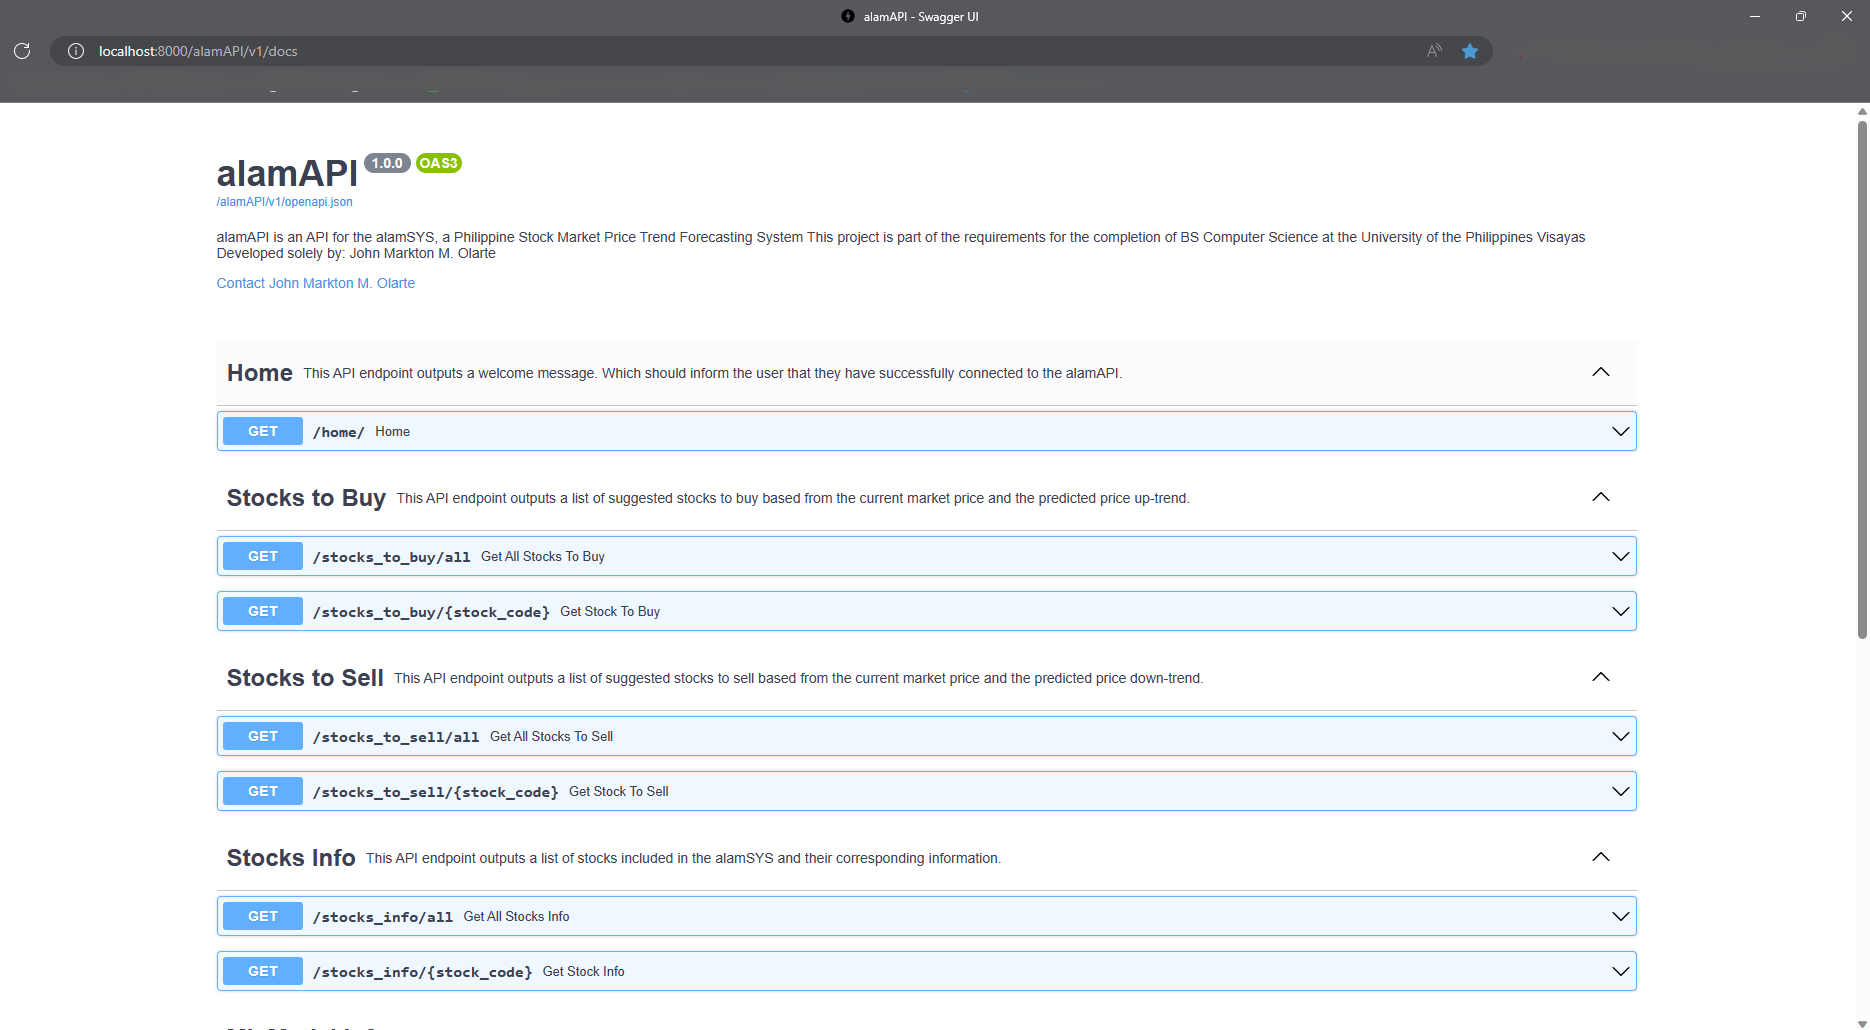
\includegraphics[width=0.85\textwidth]{./assets/Chapter_4/Documentation/alamAPI_swagger.png}
    \caption{alamAPI Web-based API Documentation Using Swagger}
    \label{fig:alamapi_swagger}
\end{figure}
\FloatBarrier

\begin{figure}[ht]
    \centering
    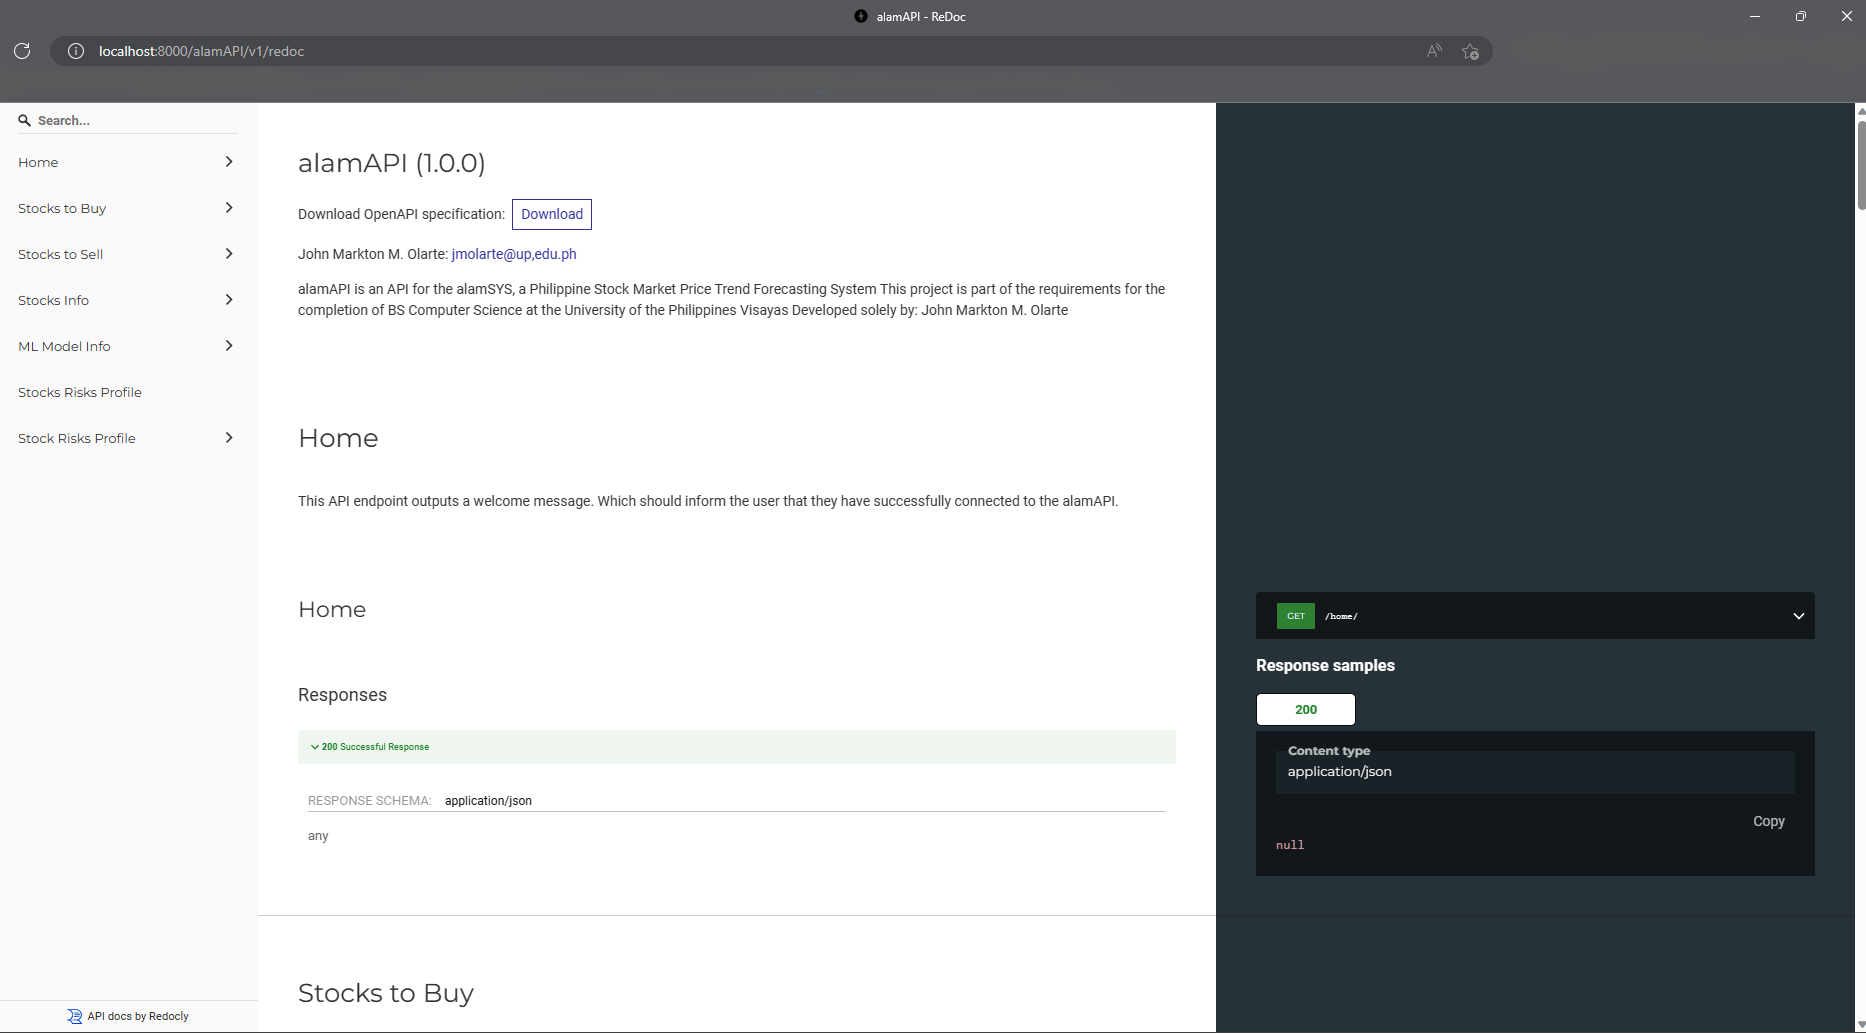
\includegraphics[width=0.85\textwidth]{./assets/Chapter_4/Documentation/alamAPI_redoc.png}
    \caption{alamAPI Web-based API Documentation Using Redocs}
    \label{fig:alamAPI_redoc}
\end{figure}
\FloatBarrier

Moving on, the Swagger-based documentation was used to show the API Endpoints. To begin, the 
'Home' refers to the API endpoint that returns a welcome message informing the API user that they 
have successfully connected to the alamAPI and that everything is functioning properly. 
Figure \ref{fig:alamAPI_home} depicts 
an example request executed using this API endpoint.
\\
\begin{figure}[ht]
    \centering
    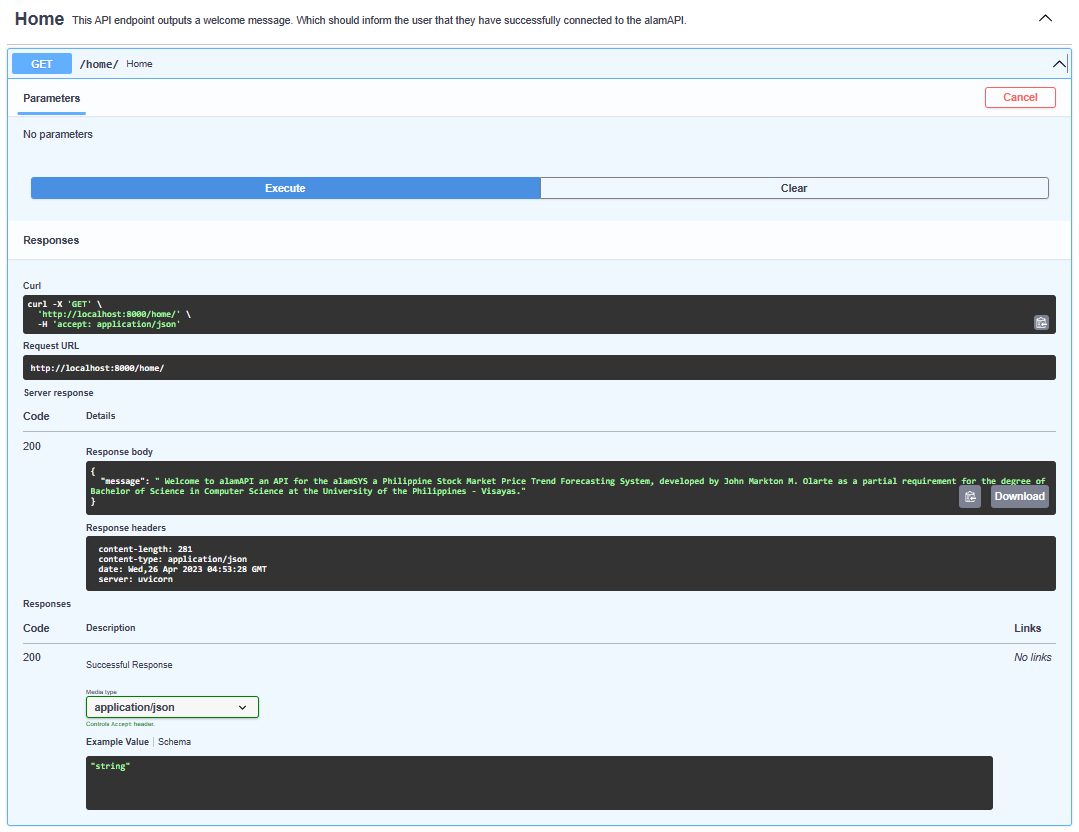
\includegraphics[width=0.85\textwidth]{./assets/Chapter_4/Documentation/alamAPI_home.png}
    \caption{Sample API Endpoint: Home Request}
    \label{fig:alamAPI_home}
\end{figure}
\FloatBarrier

Next, API endpoints related to the 'Stock to Buy', which output a list of 
suggested stocks to buy based on the current market price and the 
predicted price up-trend. This API endpoint has two uses: users can 
use the /all path to see all of the suggested stocks to buy, or 
they can use /stock\_code, which requires a specific stock code 
and returns the details for that stock if it exists in the stocks to buy list, 
and if it does not, it instead returns a 'Stock not found' alert.
A sample execution, specifically for
/all is shown is shown in Figure \ref{fig:alamAPI_buy}
\begin{figure}[ht]
    \centering
    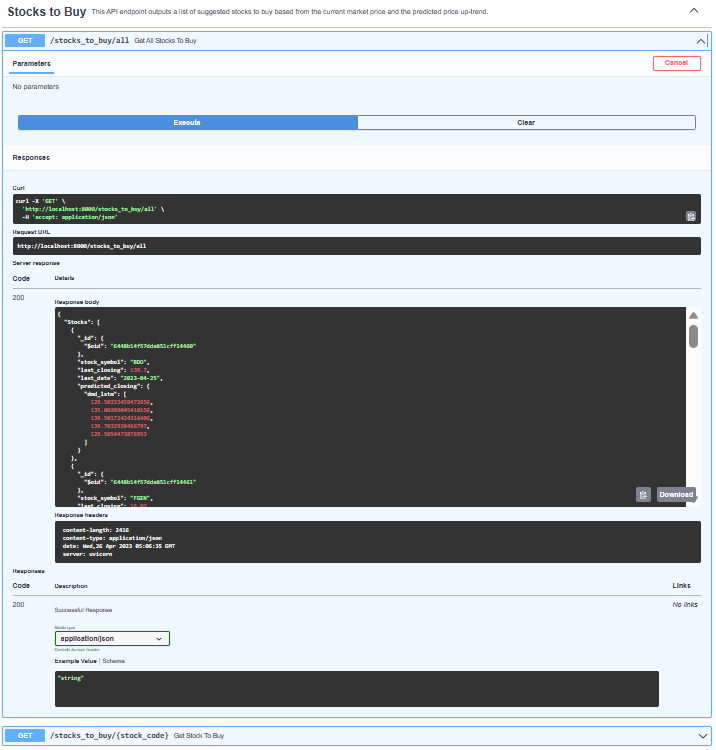
\includegraphics[width=0.85\textwidth]{./assets/Chapter_4/Documentation/alamAPI_buy.png}
    \caption{Sample API Endpoint: Buy (all) Request}
    \label{fig:alamAPI_buy}
\end{figure}
\FloatBarrier

The third set of API endpoints is related to the 'Stock to Sell,' which returns 
a list of recommended stocks to sell based on the current market price and 
the predicted price downtrend. Users can use the /all path to see all of 
the suggested stocks to sell, or they can use /stock\_code, which requires a 
specific stock code and returns the details for that stock if it exists in the 
stocks to sell list, and a 'Stock not found' alert if it does not. Figure 
\ref{fig:alamAPI_sell} shows a sample execution, specifically for /all.
\begin{figure}[ht]
    \centering
    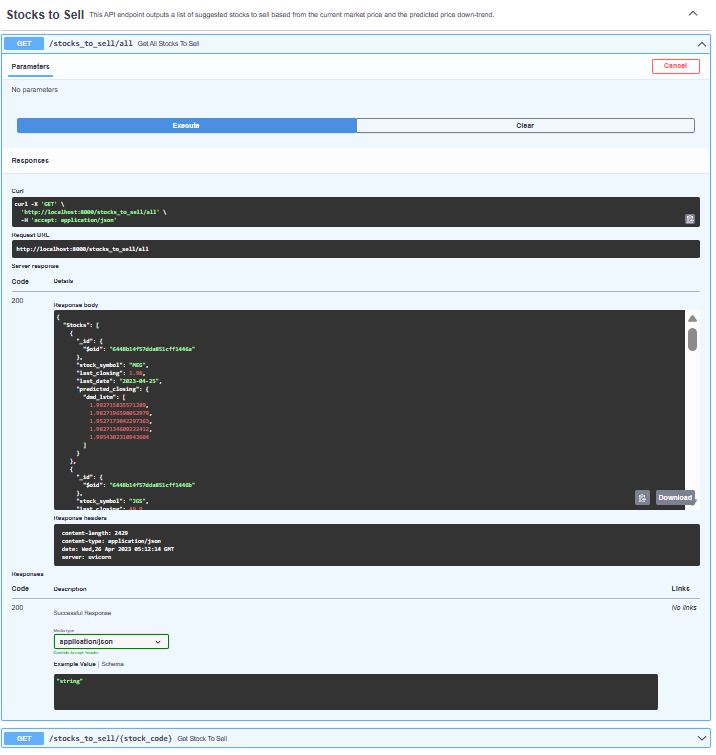
\includegraphics[width=0.85\textwidth]{./assets/Chapter_4/Documentation/alamAPI_sell.png}
    \caption{Sample API Endpoint: Sell (all) Request}
    \label{fig:alamAPI_sell}
\end{figure}
\FloatBarrier

The next set of API endpoints is related to the 'Stocks Info', which returns a 
list of stocks that are part of the alamSYS. This API endpoint has two uses: 
users can use the /all path to see information from all 20 stocks included 
in this iteration of the alamSYS, or they can use /stock\_code, which 
requires a specific stock code and returns information from that specific 
stock if it exists in the alamSYS, and a 'Stock not found' alert if it does not.
Figure \ref{fig:alamAPI_info} shows a sample execution, specifically for /all.
\begin{figure}[ht]
    \centering
    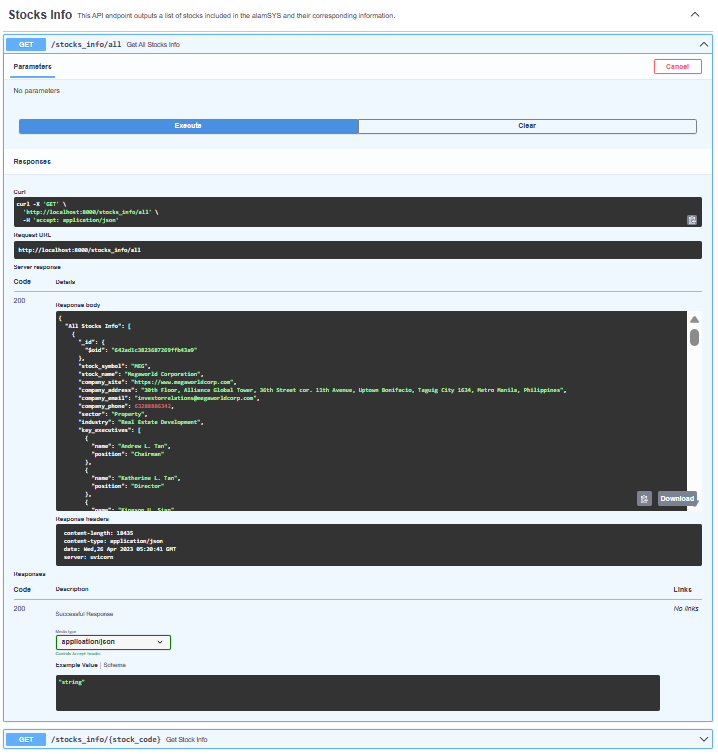
\includegraphics[width=0.85\textwidth]{./assets/Chapter_4/Documentation/alamAPI_info.png}
    \caption{Sample API Endpoint: Stocks Info (all) Request}
    \label{fig:alamAPI_info}
\end{figure}
\FloatBarrier

The fifth set of API endpoints is related to the 'ML Model Info', 
which returns a list of machine learning models that have been deployed in 
the alamSYS. In particular, in this iteration of the alamSYS, the current 
deployed deep learning model is DMD-LSTS, as discussed in previous Chapters 
of this paper. This API endpoint has two uses: users can use the /all path 
to see information for all models, or they can use /model\_name, which requires 
a model name and returns information for that specific model if it exists in 
the alamSYS, and a 'Model not found' alert if it does not. Figure 
\ref{fig:alamAPI_ml} shows a sample execution, specifically for /all.
\begin{figure}[ht]
    \centering
    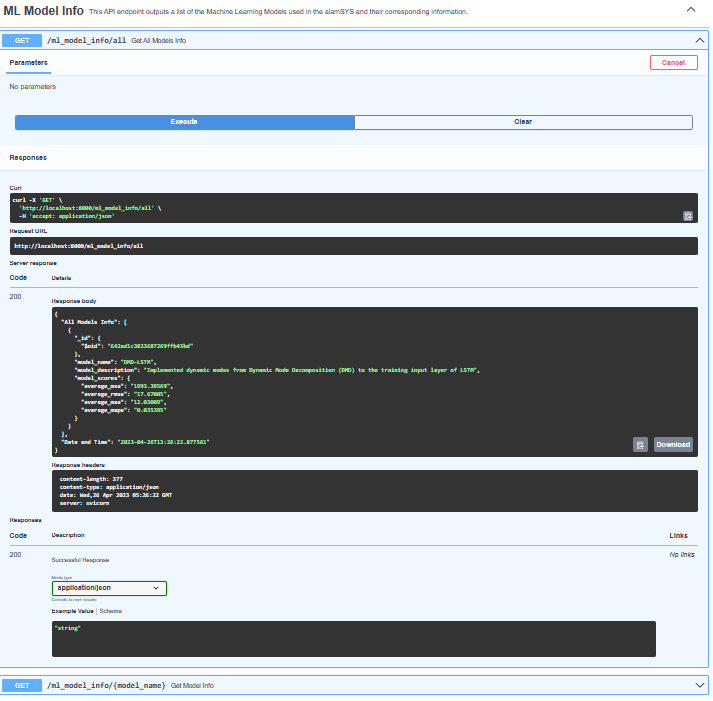
\includegraphics[width=0.85\textwidth]{./assets/Chapter_4/Documentation/alamAPI_ml.png}
    \caption{Sample API Endpoint: ML Model Info (all) Request}
    \label{fig:alamAPI_ml}
\end{figure}
\FloatBarrier


Finally, the final API endpoints related to the 'Stocks Risks Profile', 
which outputs a list of stocks in alamSYS and their corresponding risk 
values based on value at risk (\%), volatility (\%), and drawdown (\%). 
This API endpoint has two uses: users can use the /all path to see the risks 
profile information for all stocks, or they can use /stock\_name, which 
requires a stock name and returns the risks information for that specific 
stock if it exists in the alamSYS, and a 'Stock not found' alert if it 
does not. Figure \ref{fig:alamAPI_risk} depicts a sample execution, 
specifically for /all.
\begin{figure}[ht]
    \centering
    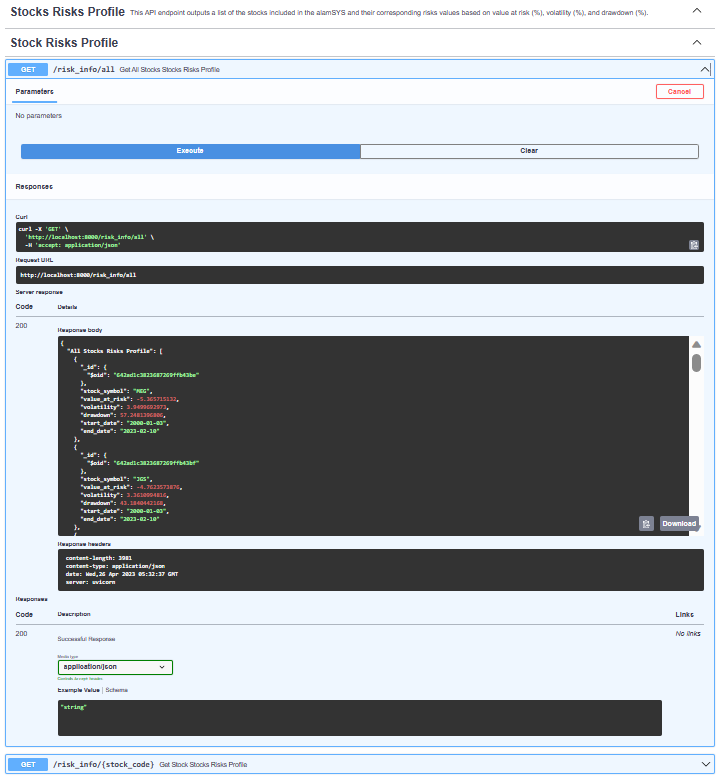
\includegraphics[width=0.85\textwidth]{./assets/Chapter_4/Documentation/alamAPI_risk.png}
    \caption{Sample API Endpoint: Stocks Risks Profile (all) Request}
    \label{fig:alamAPI_risk}
\end{figure}
\FloatBarrier

To go over the following risk values in greater detail. Furthermore, 
Table \ref{tab:risk_profiles} summarizes the risk values 
for all stocks included in the alamSYS:
\begin{itemize}
    \item[(a)] Value at Risk (VaR) is a statistic that quantifies 
    the extent of potential financial losses within a firm, 
    portfolio, or position over a specific time period, 
    and risk managers use VaR to measure and control the level 
    of risk exposure \cite{Kenton2023}.
    The alamSYS calculated the value at risk 
    based on the daily return percentage of each stock from January 
    03, 2000 to February 02, 2023, that is below 5\%. 
    In Table \ref{tab:risk_profiles} it shows a negative VaR, which means that percentile amount
    is the expected returns below 5\% is computed for that values.
    For example, PSEI shows -1.88780\% VaR which means that it
    has a 1.88780\% chance to loss 5\% of its value for the next day,
    while having 99.11220\% chance of gaining above 5\% on a 
    daily basis. Take note that the negative symbol in VaR indicates 
    the likelihood of losing in the position. 
    \item[(b)] Volatility is a statistical indicator of the spread 
    of returns for a specific security or market index. The higher 
    the volatility, in most cases, the riskier the security
    \cite{Hayes2023}.
    It was measured in the alamSYS in terms of the volatility 
    percentage based on standard deviation of daily returns of 
    each stock from January 3, 2000 to February 2, 2023.
    The data presented in Table \ref{tab:risk_profiles} shows that the 
    LTG stock is the most volatile of the stocks included in the 
    alamSYS, implying that investors or traders should keep a 
    closer eye on LTG than other stocks with volatility ranging 
    from around 1.3\% to 7\%.
    \item[(c)] Drawdown is useful for calculating the historical 
    risk of various investments, comparing fund performance, and 
    monitoring personal trading performance \cite{Mitchell2022}. 
    It was measured in the alamSYS in terms of the drawdown 
    percentage based on the maximum and minimum values of each 
    stock from data beginning January 03, 2000 until 
    February 02, 2023, essentially to measure the stock's 
    performance during that time period. The overall drawdown 
    values from the alamSYS stocks, as shown in 
    Table \ref{tab:risk_profiles}, show a 
    positive upside, but this also indicates the possibility of 
    reversed risk, where a drawdown of 50\%, for example, can 
    also mean a potential loss of 50\% of an investor's total capital.
\end{itemize}

\begin{longtable}[c]{cccc}
    \caption{Summary of Risk Profile for Each Stock in the alamSYS}
    \label{tab:risk_profiles}\\
    \hline
    \textbf{STOCK} & \textbf{\begin{tabular}[c]{@{}c@{}}VALUE AT \\ RISK\\ (\%)\end{tabular}} & \textbf{\begin{tabular}[c]{@{}c@{}}VOLATILITY \\ (\%)\end{tabular}} & \textbf{\begin{tabular}[c]{@{}c@{}}DRAWDOWN \\ (\%)\end{tabular}} \\ \hline
    \endfirsthead
    %
    \multicolumn{4}{c}%
    {{\bfseries Table \thetable\ continued from previous page}} \\
    \hline
    \textbf{STOCK} & \textbf{\begin{tabular}[c]{@{}c@{}}VALUE AT \\ RISK\\ (\%)\end{tabular}} & \textbf{\begin{tabular}[c]{@{}c@{}}VOLATILITY \\ (\%)\end{tabular}} & \textbf{\begin{tabular}[c]{@{}c@{}}DRAWDOWN \\ (\%)\end{tabular}} \\ \hline
    \endhead
    %
    \hline
    \endfoot
    %
    \endlastfoot
    %
    \textbf{MEG}   & -5.36572                                                                 & 3.94997                                                             & 57.24814                                                          \\
    \textbf{JGS}   & -4.76236                                                                 & 3.36110                                                             & 43.18404                                                          \\
    \textbf{BDO}   & -3.30249                                                                 & 2.36405                                                             & 39.67065                                                          \\
    \textbf{FGEN}  & -3.81908                                                                 & 2.55925                                                             & 30.60426                                                          \\
    \textbf{ICT}   & -4.82705                                                                 & 3.52084                                                             & 54.64501                                                          \\
    \textbf{ALI}   & -4.39048                                                                 & 3.07049                                                             & 56.02617                                                          \\
    \textbf{SMC}   & -3.40367                                                                 & 2.38596                                                             & 45.29878                                                          \\
    \textbf{TEL}   & -3.69376                                                                 & 2.46002                                                             & 44.65912                                                          \\
    \textbf{GLO}   & -4.12004                                                                 & 3.09260                                                             & 54.75806                                                          \\
    \textbf{BLOOM} & -5.98500                                                                 & 7.06155                                                             & 100.00000                                                         \\
    \textbf{RLC}   & -4.52936                                                                 & 3.41699                                                             & 65.98291                                                          \\
    \textbf{MER}   & -4.49859                                                                 & 3.25474                                                             & 76.00003                                                          \\
    \textbf{AC}    & -4.29065                                                                 & 2.79617                                                             & 46.68883                                                          \\
    \textbf{PGOLD} & -3.11492                                                                 & 2.13482                                                             & 25.79979                                                          \\
    \textbf{LTG}   & -6.15322                                                                 & 31.22332                                                            & 1667.80691                                                        \\
    \textbf{MPI}   & -4.05584                                                                 & 3.49968                                                             & 81.13252                                                          \\
    \textbf{AP}    & -3.19764                                                                 & 2.18729                                                             & 26.54088                                                          \\
    \textbf{RRHI}  & -3.03206                                                                 & 2.05393                                                             & 24.50967                                                          \\
    \textbf{URC}   & -4.53239                                                                 & 3.19972                                                             & 42.54262                                                          \\
    \textbf{PSEI}  & -1.88780                                                                 & 1.31882                                                             & 30.90366                                                          \\ \hline
\end{longtable}}

\subsubsection{alamAPI Use Case Diagram}
\label{subsubsec:use_case_diagram}
Based on the API endpoints discussed in the previous section, 
the author has illustrated the use case of the alamAPI in this section. 
Furthermore, the use case diagram in Figure \ref{fig:alamAPI_use_case} 
adheres to the Unified Modeling Language (UML) definition of a use 
case diagram as published in \citeauthor{UseCaseDiagram}'s 
\citeyear{UseCaseDiagram} guides.
\textit{Note that this only pertains to the interaction of potential
users in the alamAPI, and not to the whole alamSYS.}
\begin{figure}[ht]
    \centering
    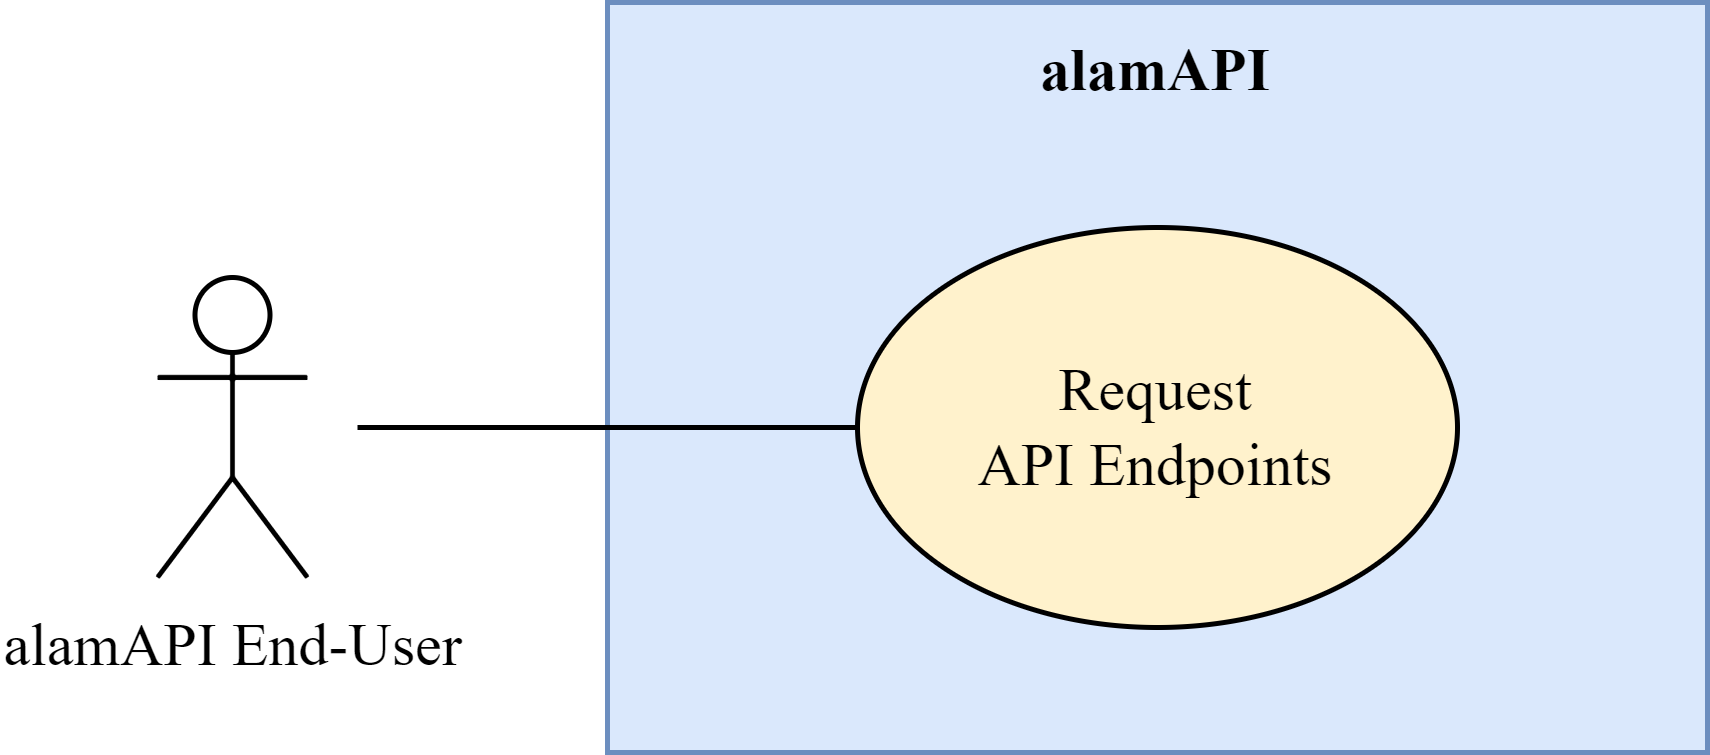
\includegraphics[width=0.85\textwidth]{./assets/Chapter_4/Documentation/alam_api_usecase.png}
    \caption{alamAPI End User UML Use Case Diagram}
    \label{fig:alamAPI_use_case}
\end{figure}
\FloatBarrier

The use case diagram above demonstrates how easy and simple it is to use the alamAPI, 
as end users are only required to create requests from the listed API endpoints.


\subsubsection{alamAPI Docker Management}
\label{subsubsec:alamAPI_docker_management}
The management and maintenance of the alamAPI container is 
also made possible through the utilization of Docker Desktop.
Figure \ref{fig:alamapi_tree} depicts the tree of files and directories accessible 
from '/alamAPI/' of the alamAPI docker container.
\begin{figure}[ht]
    \centering
    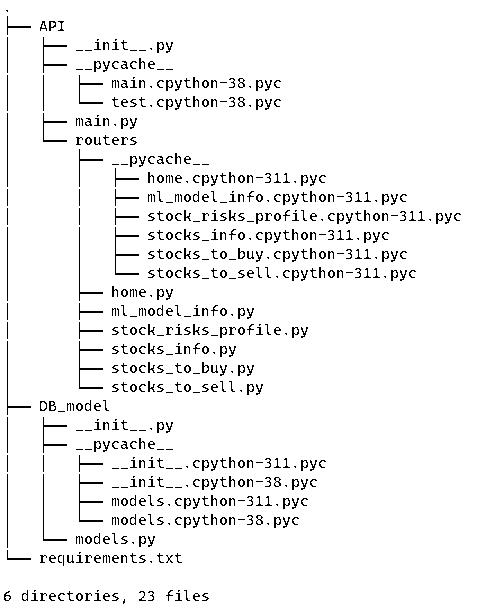
\includegraphics[height=0.45\textheight]{./assets/Chapter_4/Documentation/alamapi_tree.png}
    \caption{alamAPI Docker Container Directory Tree}
    \label{fig:alamapi_tree}
\end{figure}
\FloatBarrier

On the other hand, alamDB's docker container management only displays 
alamDB status updates, whereas direct management employs known mongoDB 
command line interface commands. 
However, utilization of CLI commands through docker desktop can be 
time-consuming for system administrators or system managers, 
so it is best to use a GUI-based mongoDB management tool, 
as discussed in the succeeding section.

\subsubsection{alamDB MongoDBCompass Management}
\label{subsubsec:alamBB_docker_management}
The use of a GUI-based database management tool for alamDB is critical 
in maintaining the system's ease of maintenance. As a result, the author 
recommends that future system administrators or maintainers use software 
such as MongoDBCompass, which is available for Windows users.

% Discuss how to use MongoDBCompass to Manage the content of the alamDB
Utilization of the MongoDBCompass is straightforward and is only composed of
these few steps:
\begin{itemize}
    \item[(a)] First, indicate a new connection using the default URI: 
    mongodb://localhost:27017.
    \item[(b)] Once the URI is initiated, press or tap the 'Connect' button
    to establish connection to the alamDB.
    \item[(c)] Finally, you have access to the alamDB. As shown in Figure
    \ref{fig:mongodb_compass} system users has the access to the following databases:
    \begin{itemize}
        \item[1.] admin - which currently have an empty collection of data
        \item[2.] alamAPI\_DB - which corresponds to the database of the alamSYS
        \item[3.] config - which is also currently empty; and 
        \item[4.] local - which contains the startup\_log collection, and whose data is autogenerated by mongoDB.
        \begin{figure}[ht]
            \centering
            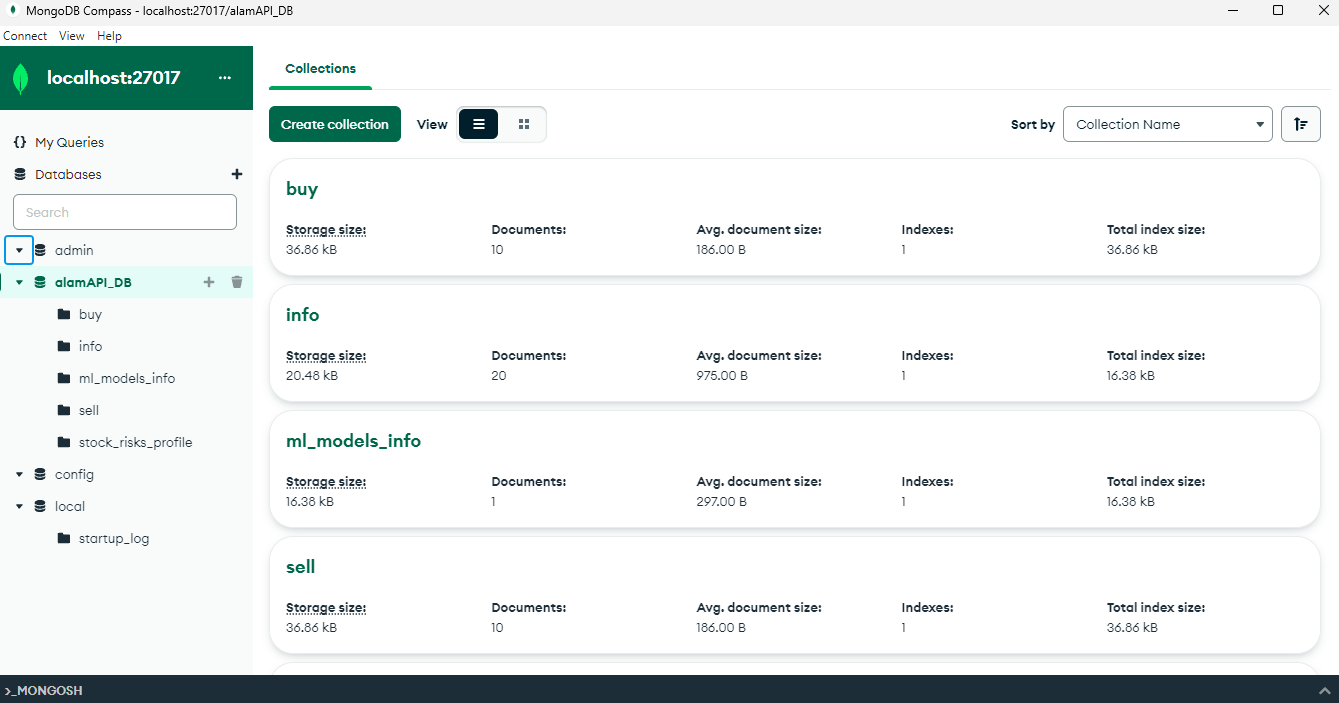
\includegraphics[width=0.85\textwidth]{./assets/Chapter_4/Documentation/mongodb_compass.png}
            \caption{MongoDB Compass Database Management of alamDB}
            \label{fig:mongodb_compass}
        \end{figure}
        \FloatBarrier
    \end{itemize}
\end{itemize}